%!TEX program = pdflatex
\documentclass[10pt]{article}
\usepackage[pdftex]{graphicx, color}
\usepackage{listings}
\usepackage{mathtools} 
\usepackage{tikz}
\usetikzlibrary{automata,positioning}

\headheight 8pt \headsep 20pt \footskip 30pt
\textheight 9in \textwidth 6.5in
\oddsidemargin 0in \evensidemargin 0in
\topmargin -.35in
\newcommand {\pts}[1]{({\bf #1 pts})}
\lstset{basicstyle=\small\ttfamily,breaklines=true}

\begin{document}
\begin{center}
\Large CS131 Compilers: Writing Assignment 1\\Due Saturday, March 13, 2021 at 23:59pm
\end{center}

\begin{center}
%% Change this:
\LARGE Feiran Qin - 2019533161
\end{center}


This assignment asks you to prepare written answers to questions on
regular languages, finite automata, and lexical analysis.  Each of the
questions has a short answer.  You may discuss this assignment with
other students and work on the problems together.  However, your
write-up should be your own individual work and you should indicate in your submission who you worked
with, if applicable.  Written assignments are turned in at the start of lecture.
You should use the Latex template provided at the course web site to write your solution and use the \emph{tikz} package to draw
automata.

\begin{center}
%% Change this:
I worked with: (Haotian Jing, 2018533233), (Yining Zhang,2019533103), (Songhui Cao,2018533156)
\end{center}

\begin{enumerate}
  \item \pts{$1\times 3=3$} For each of the follow prompts, write any non-empty sentence:
  \begin{enumerate}
           \item Name one reason why you would like to learn in this class.
            \[
                $$
                Understanding Compilers can serve for the programming of Underlying Code, which is important in learning computer science.
                $$
            \]
           \item Write a question you would like the professor to answer 1 on any topic, from personal opinions to the class material and the teaching assistant to answer 1 in the discussion part.
            \[
                $$
                I want to know more about the lowring optimization of the IR code. 
                $$
            \]
           \item What do you expect from this class.
            \[
            $$ 
            The ability of system programming and the knowledge of Programming Language.
            $$
            \]
        \end{enumerate}
  %
  \item \pts{$1\times 3=3$} Briefly explain why the following language do not have regular expression.
  \begin{enumerate}
           \item The set of all finite strings over the alphabet $\Sigma=\{a,b\}$ that the number of a is bigger than b.
            
            \[
                $$
                Regex is used for match strings. It can't be used for counting numbers of specific character and do logical calculations.
                \\
                Suppose $s = a ^ {p+k}B^p$ , which is in $s = uv^nw$ where $uv^n= a^{p+k} $. When $n=1$, the number of a can be smaller than b. Which is wrong.
                $$
                \]
           \item The set of all finite palindromic strings over the alphabet $\Sigma=\{a,b\}$ that remains the same when its digits are reversed.
            \[
            $$
                Regex expression can't determine the Symmetry point of the palindromic expression. \\
                Suppose $s = abcddcba$, which in in $s = uv^nw$ where  $u = a$ , $v = bcd$ , $n=1$ , $w=dcba$ . It's obvious that when $n <> 1$. Which is wrong.
            $$  
            \]
           \item Grammar correct C++ program.
            \[
            $$
                Regex expression can't do the jobs of Syntax Analyser and Parser. 
            $$
            \]
  \end{enumerate}

  \item \pts{$2\times 2=4$} Write regular expressions for the following languages over the alphabet $\Sigma=\{a,b,c\}$:
 \begin{enumerate}
           \item $L_1$: The set of all finite strings that the first appearing a is ahead of the first appearing b.
            \[
            $$
                $(c)^*(a)(a+c)^*(a + b + c)^*$
            $$
            \]
           \item $L_2$: The set of all finite strings containing $a's$ for even times.
            \[
            $$
                $ (b+c)^*(a(b+c)^*a)^*(b+c)^* $
            $$  
            \]
 \end{enumerate}
 \item \pts{$2\times 2=4$} Write regular expressions for the following languages over the alphabet $\Sigma=\{0,1\}$:
 \begin{enumerate}
           \item $L_3$: The set of all finite strings that is Binary number and bigger than 101001.
            \[
            $$
            $ (0^*) 1| (0|1) | (0|1) | (0|1) | (0|1)| (0|1) | (0|1)^+  ) \\
            |(0^*)1 0101(0|1) \\
            | 0^*1011(0|1)(0|1) \\
            | 0^*11 (0|1) (0|1) (0|1) (0|1) 
            $ 
            $$
            \]
           \item $L_4$: The set of all finite strings containing at least two 0's and at most three 1's
            \[
            $$
                $
                (0^+0^+)|\\
                (0^+0^+10*)| (0^+10^+) | (0*10^+0^+) | \\
                (0^+0^+10*10*) |(0*10^+0^+10*)| (0*10*10^+0^+) | (0^+10^+10*) | (0^+10*10^+) | (0*10^+10^+) |
                \\0^+0^+10*10*10*|0*10^+0^+10*10* |0*10*10^+0^+10* | 0*10*10*10^+0^+ | 0^+10^+10*10* | 0^+10*10^+10* | 0^+10*10*10^+ | 0*10^+10^+10* | 0*10^+10*10^+  | 0*10*10^+10^+ 
                $
            $$
            \]
   \end{enumerate}
   This example illustrates that regular languages are closed under intersection. Note that
   $L_3=L_1\cap L_2$.

  \newpage
   \item \pts{$2\times 4=8$} Draw DFA's for each of the languages $L_1$, $L_2$, $L_3$ and $L_4$ from Question 3 and 4.
  \begin{enumerate}
    \item $L_1$.
    \\
    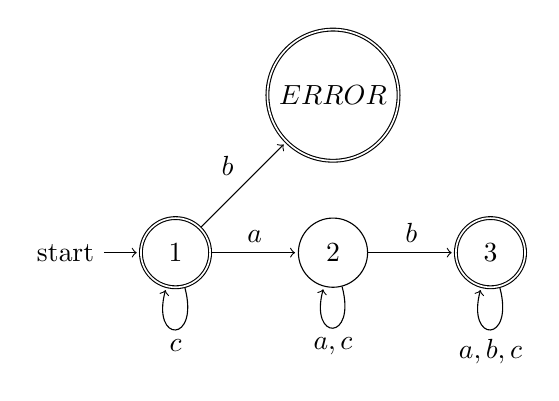
\begin{tikzpicture}[shorten >=1pt,node distance=2cm,on grid,auto]
        \node[state, initial, accepting] (1) {$1$};
        \node[state ] (2) [right= of 1]  {$2$};
        \node [state, accepting] (3) [right = of 2] {$3$};
        \node[state, accepting] (e) [above = of 2]{$ERROR$};

        \path [ ->]
        (1) edge [loop below] node {$c$} (1)
        (1) edge  node {$a$} (2)
        (2) edge [loop below] node {$a,c$} (2)
        (2) edge node {$b$} (3)
        (3) edge [loop below] node {$a,b,c$} (3)
        (1) edge node {$b$} (e);
    \end{tikzpicture}
    \item $L_2$.
    \\
    \begin{tikzpicture}[shorten >=1pt,node distance=2cm,on grid,auto]
       \node [state, initial , accepting] (a) {$1$};
       \node [state] (2) [right=of 1] {$2$};
        
        \path[ ->] 
        (1) edge [loop below] node {$b,c$} ()
        (2) edge [loop below] node {$b,c$} ()
        (1) edge [bend left] node {$a$} (2)
        (2) edge [bend left] node {$a$} (1);
    \end{tikzpicture}
    \item $L_3$.
    \\
    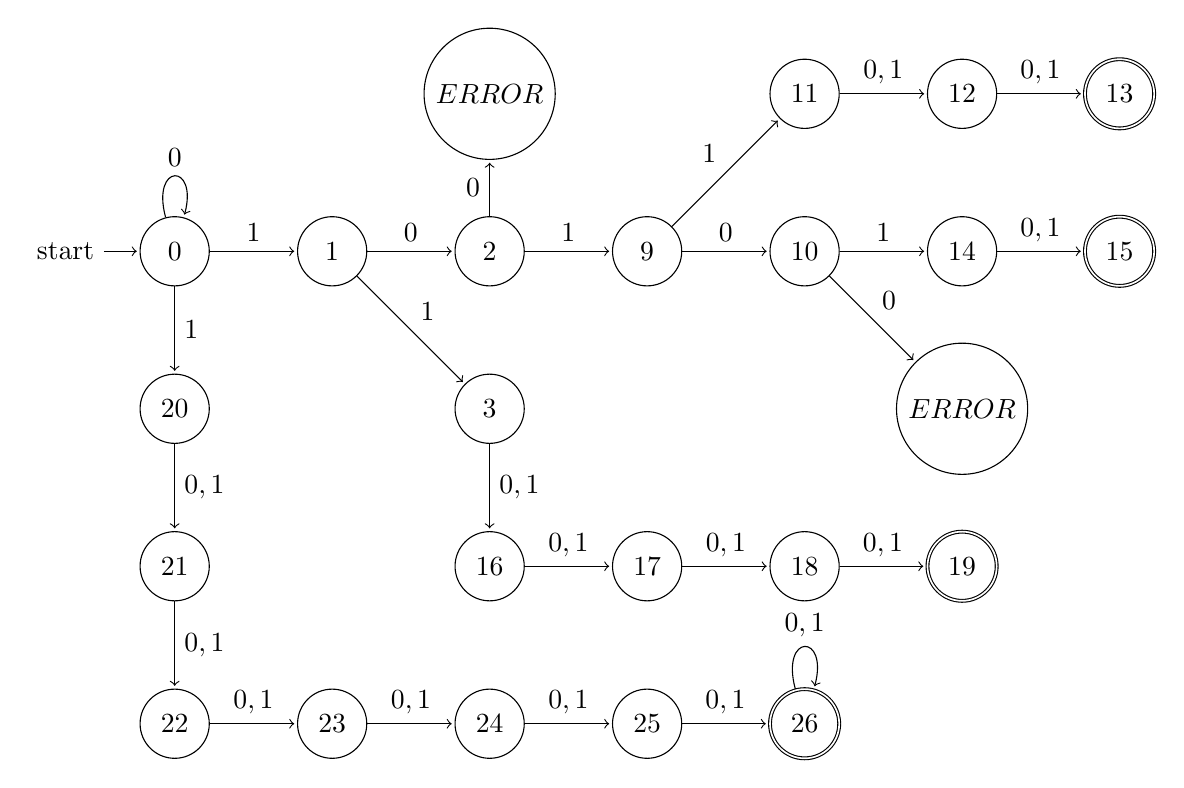
\begin{tikzpicture}[shorten >=1pt,node distance=2cm,on grid,auto]
        \node [state, initial] (0) {$0$};
        \node [state] (1)  [right =of 0]{$1$};
        \node [state] (2) [right= of 1] {$2$};
        \node [state] (3) [below = of 2] {$3$};
        \node [state] (e) [right, above = of 2] {$ERROR$};
        \node [state] (9) [right  = of 2] {$9$};
        \node [state] (10) [right = of 9] {$10$};
        \node [state] (11) [above = of 10] {$11$};
        \node [state] (12) [right = of 11] {$12$};
        \node [state, accepting] (13) [right = of 12] {$13$};
        \node [state] (14) [right = of 10] {$14$};
        \node [state] (e1) [below = of 14] {$ERROR$};
        \node [state, accepting] (15) [right = of 14] {$15$};
        \node [state] (16) [below = of 3] {$16$};
        \node [state] (17) [right = of 16] {$17$};
        \node [state] (18) [right = of 17] {$18$};
        \node [state, accepting] (19) [right = of 18] {$19$};
        \node [state] (20) [below = of 0] {$20$};
        \node [state] (21) [below = of 20] {$21$};
        \node [state] (22) [below = of 21] {$22$};
        \node [state] (23) [right = of 22] {$23$};
        \node [state] (24) [right = of 23] {$24$};
        \node [state] (25) [right = of 24] {$25$};
        \node [state, accepting] (26) [right = of 25] {$26$};
        
        \path[->]
        (0) edge [loop above] node {$0$} ()
        (0) edge node {$1$} (1)
        (1) edge node {$0$} (2)
        (1) edge node {$1$} (3)
        (2) edge node {$0$} (e)
        (2) edge node {$1$} (9)
        (9) edge node {$0$} (10)
        (9) edge node {$1$} (11)
        (11) edge node {$0,1$} (12)
        (12) edge node {$0,1$} (13)
        (10) edge node {$1$} (14)
        (10) edge node {$0$} (e1)
        (14) edge node {$0,1$} (15)
        (3) edge node {$0,1$} (16)
        (16) edge node {$0,1$} (17)
        (17) edge node {$0,1$} (18)
        (18) edge node {$0,1$} (19)
        (0) edge node {$1$} (20)
        (20) edge node {$0,1$} (21)
        (21) edge node {$0,1$} (22)
        (22) edge node {$0,1$} (23)
        (23) edge node {$0,1$} (24)
        (24) edge node {$0,1$} (25)
        (25) edge node {$0,1$} (26)
        (26) edge [loop above] node {$0,1 $} ()
        ;

    \end{tikzpicture}
     \item $L_4$.
    \\
    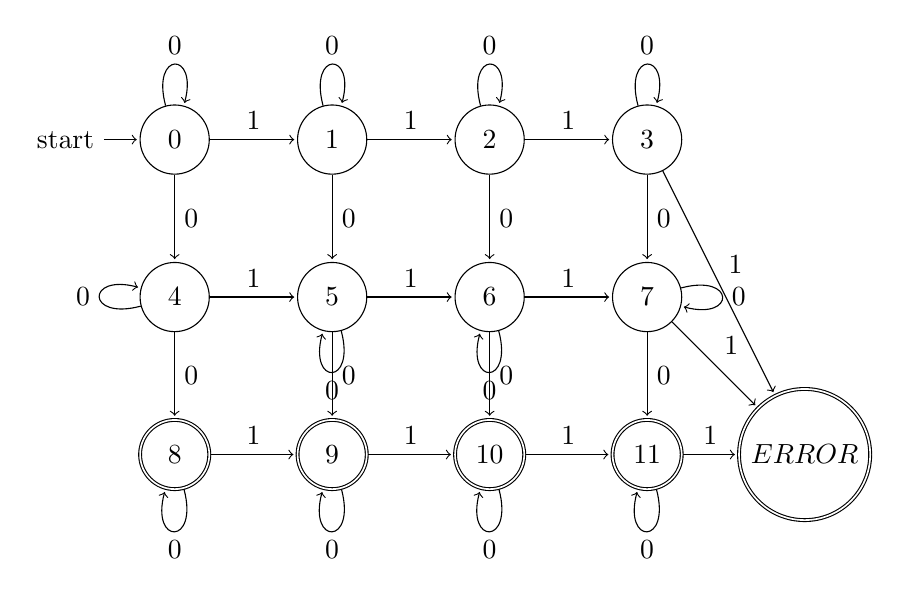
\begin{tikzpicture}[shorten >=1pt,node distance=2cm,on grid,auto]
        \node [state, initial] (0)  {$0$};
        \node [state] (1) [right=of 0]{$1$} ;
        \node [state] (2) [right=of 1]{$2$};
        \node [state] (3) [right= of 2] {$3$};
        \node [state] (4) [below= of 0] {$4$} ;
        \node [state] (5) [right= of 4] {$5$};
        \node [state] (6) [right= of 5] {$6$};
        \node [state] (7) [right= of 6] {$7$};
        \node [state, accepting] (8) [below = of 4] {$8$};
        \node [state, accepting] (9) [below = of 5] {$9$};
        \node [state, accepting] (10) [below= of 6] {$10$};
        \node [state, accepting] (11) [below = of 7] {$11$};
        \node [state, accepting] (e) [right = of 11] {$ERROR$};

    \path[->]
    (0) edge  node {$1$} (1)
    (1) edge node {$1$} (2)
    (2) edge node {$1$} (3)
    (4) edge node { $1$} (5)
    (5) edge node {$1$} (6)
    (6) edge node {$1$} (7)
    (8) edge node {$1$} (9)
    (9) edge node {$1$} (10)
    (10) edge node {$1$} (11)
    (0) edge node {$0$} (4)
    (4) edge node {$0$} (8)
    (1) edge node {$0$} (5)
    (5) edge node {$0$} (9)
    (2) edge node {$0$} (6)
    (6) edge node {$0$} (10)
    (3) edge node {$0$} (7)
    (7) edge node {$0$} (11)
    (0) edge [loop above] node {$0$} ()
    (1) edge [loop above] node {$0$} ()
    (2) edge [loop above] node {$0$} ()
    (3) edge [loop above] node {$0$} ()
    (4) edge [loop left] node {$0$} ()
    (5) edge [loop below] node {$0$} ()
    (6) edge [loop below] node {$0$} ()
    (7) edge [loop right] node {$0$} ()
    (8) edge [loop below] node {$0$} ()
    (9) edge [loop below] node {$0$} ()
    (10) edge [loop below] node {$0$} ()
    (11) edge [loop below] node {$0$} ()
    (11) edge node {$1$} (e) 
    (7) edge node {$1$} (e) 
    (3) edge node {$1$} (e)   ;

    \end{tikzpicture}
  \end{enumerate}

   \newpage


  \item \pts{$5\times 3=15$} Using the techniques covered in class, transform the following NFAs with $\epsilon$-transitions over the given alphabet $\Sigma$ into minimized DFAs. Note that a DFA must have a transition defined for every state and symbol pair, whereas a NFA need not. You must take this fact into account for your transformations. If you can't make it and write down the intermediate process, you will gain some of the score. 
  \\
  Hint: Is there a subset of states the NFA transitions to when fed a symbol for which the set of current states has no explicit transition?

  \begin{enumerate}
    \item Original NFA, $\Sigma = \{a, b, c\}$:
    \\
    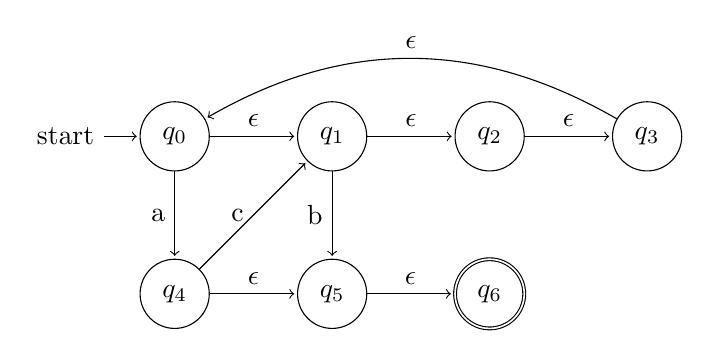
\begin{tikzpicture}[shorten >=1pt,node distance=2cm,on grid,auto]
        \node[state,initial] (q_0)   {$q_0$};
        \node[state] (q_1) [right=of q_0] {$q_1$};
        \node[state] (q_2) [right=of q_1] {$q_2$};
        \node[state] (q_3) [right=of q_2] {$q_3$};
        \node[state] (q_4) [below=of q_0] {$q_4$};
        \node[state] (q_5) [right=of q_4] {$q_5$};
        \node[state,accepting] (q_6) [right=of q_5] {$q_6$};
        \path[->]
        (q_0) edge  node {$\epsilon$} (q_1)
              edge  node  [left] {a} (q_4)
        (q_1) edge  node  {$\epsilon$} (q_2)
              edge  node  [left] {b} (q_5)
        (q_2) edge  node  {$\epsilon$} (q_3)
        (q_3) edge  [bend right] node  [above]{$\epsilon$} (q_0)
        (q_4) edge  node  [left] {c} (q_1)
                edge  node  {$\epsilon$} (q_5)
        (q_5) edge  node   {$\epsilon$} (q_6);

    \end{tikzpicture}
    \\
    Minimized DFA:
    \\
    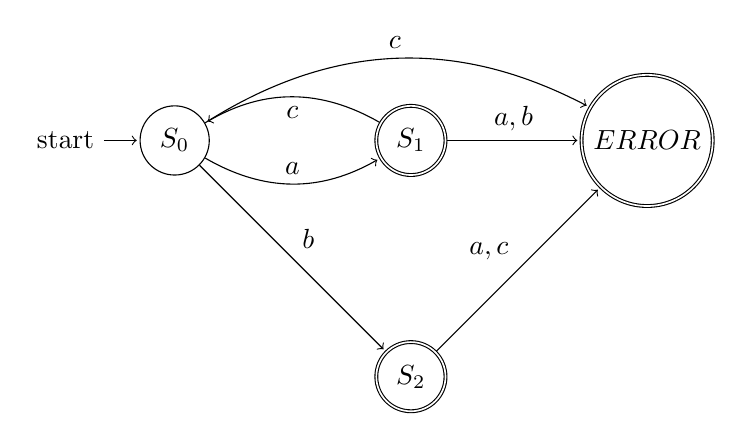
\begin{tikzpicture}[shorten >=1pt,node distance=3cm,on grid,auto]
        \node [state, initial] (0) {$S_0$};
        \node [state, accepting] (1) [right= of 0]{$S_1$};
        \node [state, accepting] (2) [below = of 1]{$S_2$};
        \node [state, accepting] (e) [right = of 1]{$ERROR$};
        \path[->]
        (0) edge  [bend right]  node {$a$} (1)
        (0) edge node {$b$} (2)
        (1) edge [bend right] node {$c$} (0)
        (1) edge node {$a,b$} (e)
        (0) edge [bend left] node [above]{$c$} (e)
        (2) edge node {$a,c$} (e)
        ;

    \end{tikzpicture}
    \item Original NFA, $\Sigma = \{a, b, c\}$:
    \\
    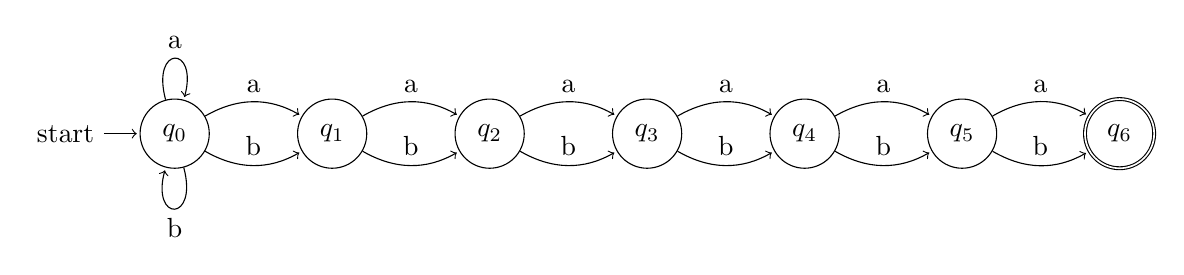
\begin{tikzpicture}[shorten >=1pt,node distance=2cm,on grid,auto]
        \node[state,initial] (q_0)   {$q_0$};
        \node[state] (q_1) [ right=of q_0] {$q_1$};
        \node[state] (q_2) [ right=of q_1] {$q_2$};
        \node[state] (q_3) [ right=of q_2] {$q_3$};
        \node[state] (q_4) [ right=of q_3] {$q_4$};
        \node[state] (q_5) [ right=of q_4] {$q_5$};
        \node[state,accepting] (q_6) [ right=of q_5] {$q_6$};
        \path[->]
        (q_0) edge [loop above] node {a} ()
              edge [loop below] node {b} ()
              edge [bend left] node  {a} (q_1)
              edge [bend right] node  {b} (q_1)
        (q_1) edge [bend left] node  {a} (q_2)
        edge [bend right] node  {b} (q_2)
        (q_2) edge [bend left] node  {a} (q_3)
        edge [bend right] node  {b} (q_3)
        (q_3) edge [bend left] node  {a} (q_4)
        edge [bend right] node  {b} (q_4)
        (q_4) edge [bend left] node  {a} (q_5)
        edge [bend right] node  {b} (q_5)
        (q_5) edge [bend left] node  {a} (q_6)
              edge [bend right] node  {b} (q_6)  ;
    \end{tikzpicture}
    \\
    Minimized DFA:
    \\
    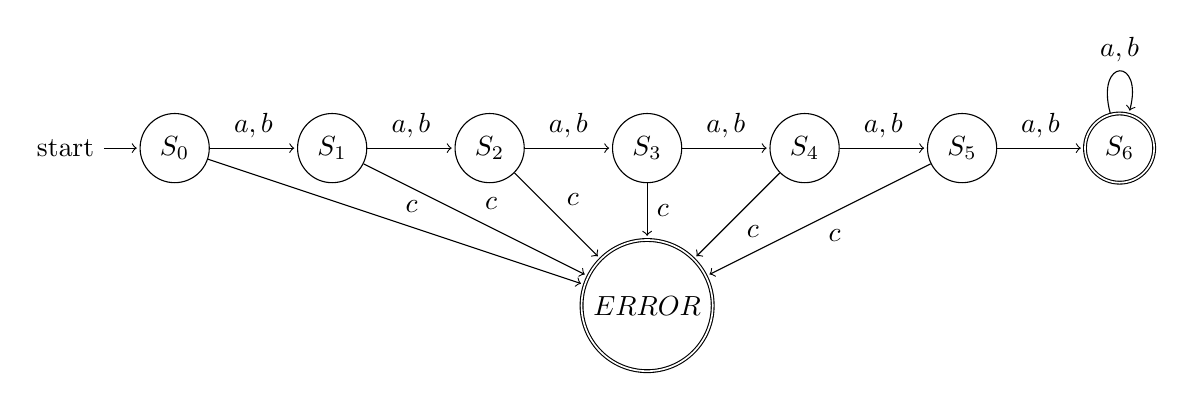
\begin{tikzpicture}[shorten >=1pt,node distance=2cm,on grid,auto]
        \node [initial, state] (0) {$S_0$};
        \node [state] (1)[right= of 0] {$S_1$};
        \node [state] (2)[right= of 1] {$S_2$};
        \node [state] (3)[right= of 2] {$S_3$};
        \node [state] (4)[right= of 3] {$S_4$};
        \node [state] (5)[right= of 4] {$S_5$};
        \node [state, accepting] (6)[right= of 5] {$S_6$};
        \node [state, accepting] (e) [below = of 3] {$ERROR$};
        \path[->]
        (0) edge node {$a,b$} (1)
        (1) edge node {$a,b$} (2)
        (2) edge node {$a,b$} (3)
        (3) edge node {$a,b$} (4)
        (4) edge node {$a,b$} (5)
        (5) edge node {$a,b$} (6)
        (6) edge [loop above] node {$a,b$} ()
        (0) edge node {$c$} (e)
        (1) edge node {$c$} (e)
        (2) edge node {$c$} (e)
        (3) edge node {$c$} (e)
        (4) edge node {$c$} (e)
        (5) edge node {$c$} (e)
        ;
    \end{tikzpicture}
    \item Original NFA, $\Sigma = \{a, b,c\}$:
    \\
    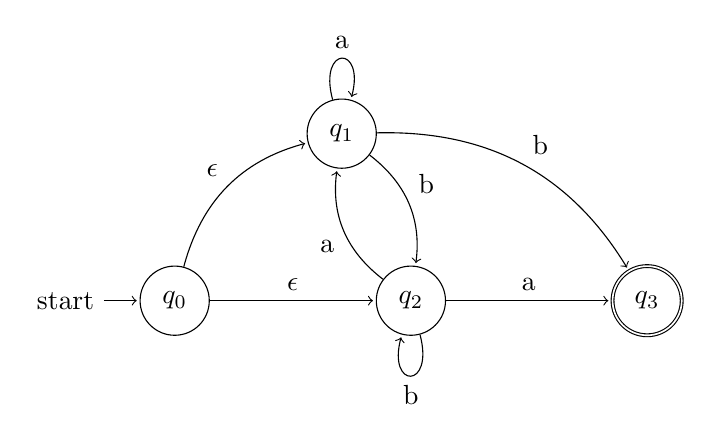
\begin{tikzpicture}[shorten >=1pt,node distance=3cm,on grid,auto]
        \node[state,initial] (q_0)   {$q_0$};
        \node[state] (q_1) [above right=of q_0] {$q_1$};
        \node[state] (q_2) [right=of q_0] {$q_2$};
        \node[state,accepting] (q_3) [right=of q_2] {$q_3$};
        \path[->]
        (q_0) edge [bend left] node  {$\epsilon$} (q_1)
              edge node  {$\epsilon$} (q_2)
        (q_1) edge [loop above] node {a} ()
              edge [bend left] node {b} (q_3)
              edge [bend left] node {b} (q_2)
        (q_2) edge [loop below] node {b} ()
              edge node {a} (q_3)
              edge [bend left] node {a} (q_1);
    \end{tikzpicture}
    \\
    Minimized DFA:
    \\
    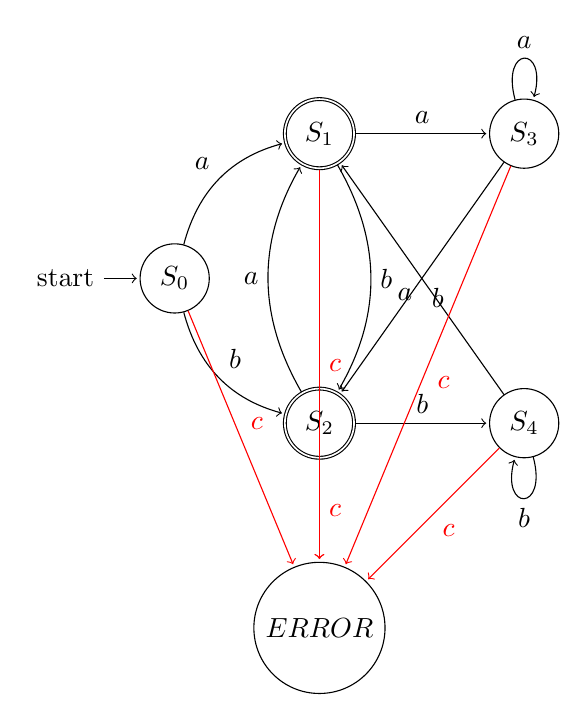
\begin{tikzpicture}[shorten >=1pt,node distance=2.6cm,on grid,auto]
        \node [initial, state] (0) {$S_0$};
        \node [state, accepting] (1) [above right = of 0]{$S_1$};
        \node [state, accepting] (2) [below right = of 0]{$S_2$};
        \node [state] (3) [ right = of 1]{$S_3$};
        \node [state] (4) [ right = of 2]{$S_4$};
        \node [state] (e) [ below = of 2]{$ERROR$};
        \path[->]
        (0) edge [bend left] node {$a$} (1)
        (0) edge [bend right] node {$b$} (2)
        (1) edge [bend left] node {$b$} (2)
        (2) edge [bend left] node {$a$}  (1)
        (1) edge node {$a$} (3)
        (2) edge node {$b$} (4)
        (3) edge node {$b$} (2)
        (4) edge node {$a$} (1)
        (3) edge [loop above] node {$a$} ()
        (4) edge [loop below] node {$b$} ()
        (0) edge [color = red]node {$c$} (e)
        (1) edge [color = red]node {$c$} (e)
        (2) edge [color = red]node {$c$} (e)
        (3) edge [color = red]node {$c$} (e)
        (4) edge [color = red]node {$c$} (e)
        ;
    \end{tikzpicture}
  \end{enumerate}

   \newpage
  \item \pts{$13$} Draw the NFA for the set of all strings over the alphabet $\Sigma = \{a,b\}$, where either $a$ occurs
an odd number of times and each of pair of a's is separated by exactly $2n+2$ consecutive b's (for some $n \geq 0$), or $b$ occurs
an even number of times and each of pair of relative consecutive b's is separated by exactly $2m+1$ consecutive a's (for some $m \geq 0$).
\\
Examples of strings that should be accepted by this NFA: abbabbbba, babaaabaaaaab.
Examples of strings that should \textbf{not} be accepted: ababb, abbbabba.
    \\
    \\
    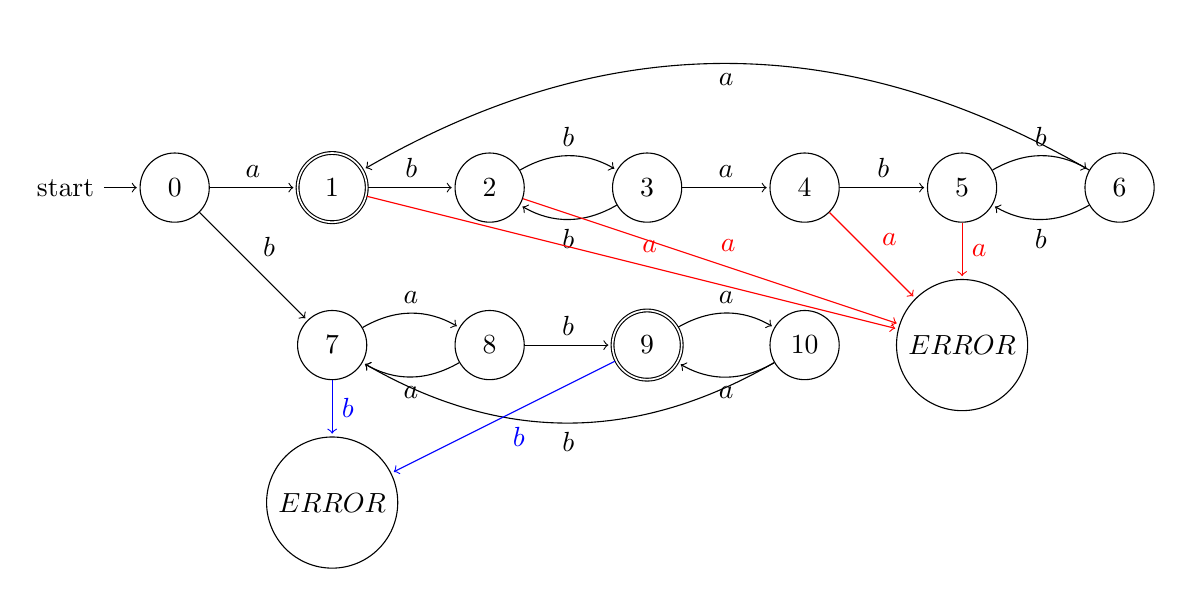
\begin{tikzpicture}[shorten >=1pt,node distance=2cm,on grid,auto]
        \node [initial, state] (0) {$0$};
        \node [state, accepting] (1) [right = of 0]{$1$};
        \node [state] (2) [right = of 1]{$2$};
        \node [state] (3) [right = of 2]{$3$};
        \node [state] (4) [right = of 3]{$4$};
        \node [state] (5) [right = of 4]{$5$};
        \node [state] (6) [right = of 5]{$6$};
        \node [state] (7) [below = of 1]{$7$};
        \node [state] (8) [right = of 7]{$8$};
        \node [state, accepting] (9) [right = of 8]{$9$};
        \node [state] (10) [right = of 9]{$10$};
        \node [state] (e) [right = of 10]{$ERROR$};
        \node [state] (e1) [below = of 7]{$ERROR$};
        \path [->]
        (0) edge node {$a$} (1)
        (1) edge node {$b$} (2)
        (2) edge [bend left] node {$b$} (3)
        (3) edge [bend left] node {$b$} (2)
        (3) edge node {$a$} (4)
        (4) edge node {$b$} (5)
        (5) edge [bend left] node {$b$} (6)
        (6) edge [bend left] node {$b$} (5)
        (6) edge [bend right] node {$a$} (1)
        (0) edge node {$b$} (7)
        (7) edge [bend left] node {$a$} (8)
        (8) edge [bend left] node {$a$} (7)
        (8) edge node {$b$} (9)
        (9) edge [bend left] node {$a$} (10)
        (10) edge [bend left] node {$a$} (9)
        (10) edge [bend left] node {$b$} (7)

        (1) edge [color = red] node {$a$} (e)
        (2) edge [color = red] node {$a$} (e)
        (4) edge [color = red] node {$a$} (e)
        (5) edge [color = red] node {$a$} (e)
        (7) edge [color = blue] node {$b$} (e1)
        (9) edge [color = blue] node {$b$} (e1)
        ;
    \end{tikzpicture}

      \newpage
      \item \pts{$10$} \textbf{Flex} scanner is very good tools to use, it can easily solve the problem listed above and do good error handling. The teaching assistant is recently facing a big bug when dealing with the indentation of a python parser. Please help him.
      \\
      \
      As we discussed in the lecture, the input buffer is the size of 4096 Bytes by default and we have 2 of them to take care of the lookahead safely. However, the both buffer will take in the \textbf{eof} and emit the \textbf{eof} twice. \textbf{eof} means the character is the end of the file.

      \begin{center}
        \begin{tabular}{|l|l|l|l|l|l|l|l|}
          \hline
          E &  & \small{=} & & M & $ * $ & 2 & \small{\textbf{eof}} \\
          \hline
        \end{tabular}
        \end{center}
      
        \begin{center}
            \begin{tabular}{llllllll}
              
            &  &           & &   &$\quad \quad\ \uparrow$  &     & $\ \uparrow$ \\
            &  &           & &   & $\text{lexemeBegin} $  &     &  \text{forword}\\
            \end{tabular}
            \end{center}
In the \textbf{Flex}, we have something like below, the forword will touch the eof twice, and if you write something in the \textbf{EOF} block, it will be called twice. In python, we have to call the dedent when end of file but only once. 
        \begin{lstlisting}[language = c]
switch ( *forward++ ) { 
case eof:
    if (forward is at end of first buffer ) { 
        reload second buffer;
        forward = beginning of second buffer;
    }else if (forward is at end of second buffer ) { 
        reload first buffer;
        forward = beginning of first buffer;
    }else /* eof within a buffer marks the end of input */ 
        terminate lexical analysis;
    break;
Cases for the other characters
}
        \end{lstlisting}

In terms of two buffer design of \textbf{Flex}, we can't write the code like below, thus we have to modify it to a right one, please do the modification to avoid the second eof be read so that the \textbf{EOF} block will only read once. You can test it in the program yourself.
\begin{lstlisting}
#include <stack>
#include <iostream>
#define LITERAL(type) {  std::cout << #type; return TOKEN_##type; }
std::stack<int> stack_indent;

%%

%{
  /* Init indent stack_indent */
  if (stack_indent.empty()) {
    stack_indent.push(0);
  }
%}
/* Other Lexical rules here. */
<<EOF>>   {
    while(stack_indent.top() != 0) {
          stack_indent.pop();
          LITERAL(DEDENT);
    }
    yyterminate();
}
\end{lstlisting}

% Your answer here
\begin{lstlisting}
    %x /* Some state defined here */
    %%

    <<EOF>> {

    while(stack_indent.top() != 0){
        stack_indent.pop();
        LITERAL(DEDENT);
	}
		yyterminate();
}
    \end{lstlisting}

    \end{enumerate}
\end{document}

